\documentclass[UTF8,a4paper,zihao=-4]{ctexart}
\usepackage[left=2.4cm,right=2.4cm,top=2.5cm,bottom=2.5cm]{geometry}
\usepackage{graphicx}
\usepackage{booktabs}
\usepackage{array}
\usepackage{longtable}
\usepackage{xcolor}
\usepackage{listings}
\usepackage{hyperref}
\usepackage{fancyhdr}
\usepackage{caption}
\usepackage{enumitem}
\usepackage{float}

\definecolor{navy}{HTML}{17324D}
\definecolor{blue}{HTML}{1677FF}
\definecolor{light}{HTML}{F3F6F9}
\hypersetup{colorlinks=true,linkcolor=blue,urlcolor=blue,citecolor=blue}
\captionsetup{font=small,labelfont=bf}
\setlength{\parindent}{2em}
\setlength{\parskip}{0.25em}
\pagestyle{fancy}
\fancyhf{}
\fancyhead[L]{实验一：实验基础工具使用}
\fancyhead[R]{科研工具与规范实践}
\fancyfoot[C]{\thepage}
\renewcommand{\headrulewidth}{0.4pt}

\lstset{
  basicstyle=\ttfamily\small,
  keywordstyle=\color{blue}\bfseries,
  commentstyle=\color{gray},
  stringstyle=\color{teal},
  backgroundcolor=\color{light},
  frame=single,
  rulecolor=\color{gray!30},
  breaklines=true,
  columns=fullflexible,
  showstringspaces=false,
  numbers=left,
  numberstyle=\tiny\color{gray},
  xleftmargin=1.6em,
  framexleftmargin=1.2em
}

\begin{document}

\begin{titlepage}
  \centering
  \vspace*{2.2cm}
  {\Huge\bfseries 实验一：实验基础工具使用\par}
  \vspace{0.7cm}
  {\Large Git、Codex、CC Switch 与 LaTeX 实践\par}
  \vspace{2.2cm}
  \renewcommand{\arraystretch}{1.8}
  \begin{tabular}{>{\bfseries}r l}
    姓名： & \underline{\hspace{7cm}} \\
    学号： & \underline{\hspace{7cm}} \\
    班级： & \underline{\hspace{7cm}} \\
    日期： & 2026 年 9 月 23 日 \\
  \end{tabular}
  \vfill
  {\large 实验报告\par}
\end{titlepage}

\tableofcontents
\newpage

\section{实验目标}

本实验旨在掌握科研项目的基础工具链：使用 Git 管理代码版本，理解 GitHub 远程协作流程；使用 Codex 完成一次可验证的代码生成与修改任务；了解 CC Switch 的安装、供应商配置与安全边界；使用 LaTeX 编写结构化实验报告，并通过规范的图题、标签和正文引用插入矢量实验结果图。

\section{实验环境与安全原则}

\begin{table}[H]
  \centering
  \caption{实验环境}
  \label{tab:env}
  \begin{tabular}{lll}
    \toprule
    项目 & 版本或状态 & 说明 \\
    \midrule
    操作系统 & Windows & PowerShell 环境 \\
    Git & 2.50.0.windows.2 & 已完成本地提交、推送与拉取演练 \\
    Python & 3.12.14 & 用于运行词频程序和自动测试 \\
    Codex CLI & 0.154.0-alpha.6.2 & 已安装；CLI 当前未登录 \\
    Codex 桌面应用 & 当前会话可用 & 用于本次代码生成、运行和报告整理 \\
    CC Switch & 3.20.4 Portable & 官方 Release 便携版，可执行文件已验证 \\
    XeLaTeX & MiKTeX & 用于编译本报告 \\
    \bottomrule
  \end{tabular}
\end{table}

图~\ref{fig:environment} 是经过脱敏的环境检查记录。实验过程中没有把 API Key、访问令牌、邮箱或 Codex 的 \texttt{auth.json} 写入仓库。OpenAI 官方文档说明，Codex 支持 ChatGPT 登录和 API Key 登录；用户级配置位于 \texttt{\textasciitilde/.codex/config.toml}，项目配置仅应在受信任项目中加载。\footnote{OpenAI Codex Authentication: \url{https://learn.chatgpt.com/docs/auth}；Config basics: \url{https://learn.chatgpt.com/docs/config-file/config-basic}。访问日期：2026-09-23。}

\begin{figure}[H]
  \centering
  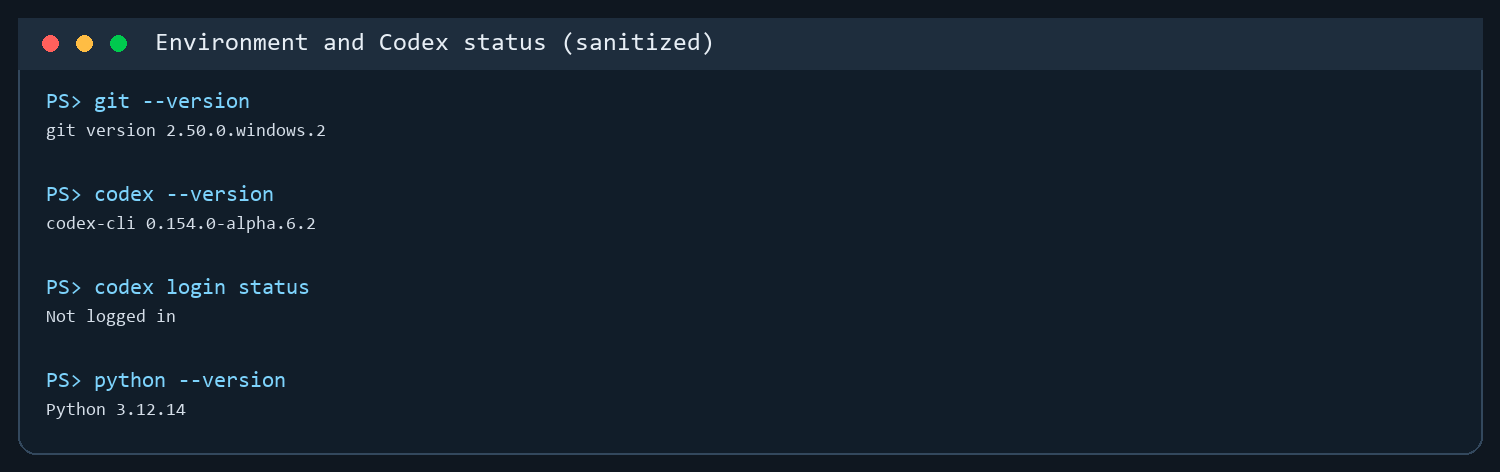
\includegraphics[width=0.93\textwidth]{../evidence/01_environment.png}
  \caption{Git、Python 与 Codex 环境检查（已脱敏）}
  \label{fig:environment}
\end{figure}

\section{LaTeX 图片排版实验}

\subsection{位图与矢量图的选择}

位图由固定像素组成，放大后容易出现锯齿；矢量图保存线条、文字和几何对象，缩放后仍可保持清晰。本实验将词频结果保存为 PDF 矢量柱状图，并统一放在 \texttt{report/figures} 目录。LaTeX 中通过 \texttt{graphicx} 宏包插图，使用 \texttt{caption} 给出图题，使用 \texttt{label} 和 \texttt{ref} 建立正文交叉引用。

\begin{lstlisting}[language={[LaTeX]TeX},caption={LaTeX 图片插入与引用代码}]
\usepackage{graphicx}
\begin{figure}[htbp]
  \centering
  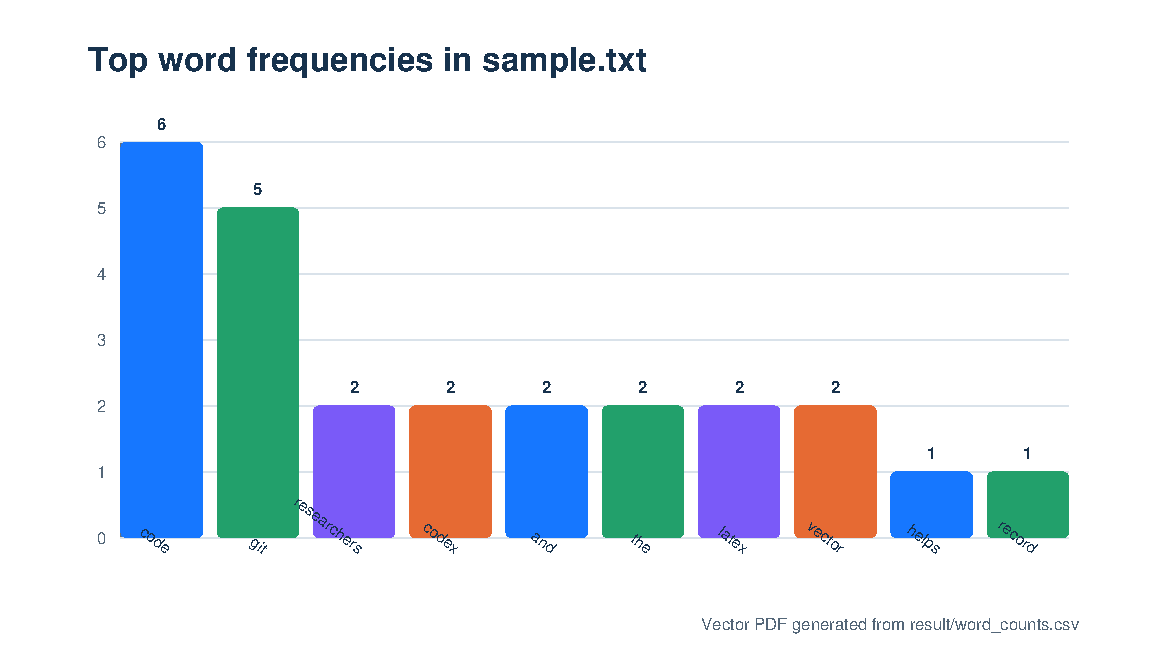
\includegraphics[width=0.86\textwidth]{figures/result.pdf}
  \caption{样例文本中出现次数最多的词}
  \label{fig:result}
\end{figure}
如图~\ref{fig:result} 所示，code 和 git 的出现次数最高。
\end{lstlisting}

\begin{figure}[H]
  \centering
  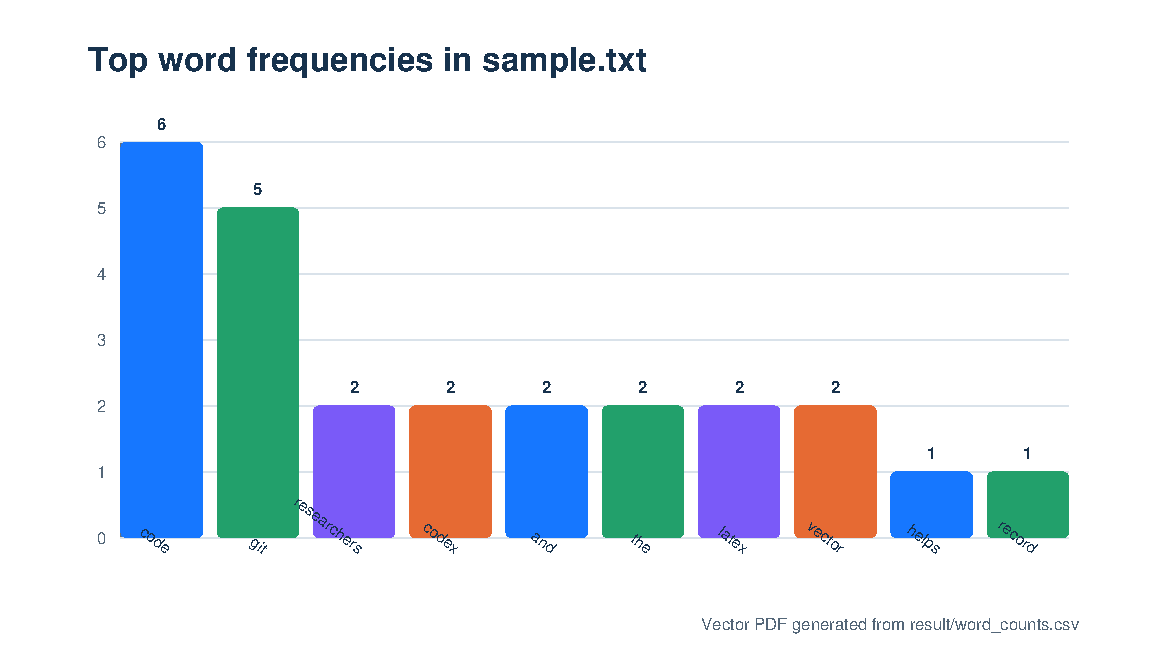
\includegraphics[width=0.86\textwidth]{figures/result.pdf}
  \caption{样例文本中出现次数最多的词（PDF 矢量图）}
  \label{fig:result}
\end{figure}

如图~\ref{fig:result} 所示，\texttt{code} 出现 6 次，\texttt{git} 出现 5 次；其余高频词出现 1--2 次。图像使用 \texttt{width=0.86\textbackslash textwidth} 控制宽度，因此能够随版心缩放且不超出页边距。

\section{Git 与远程仓库流程}

\subsection{仓库结构}

仓库按功能划分为 \texttt{code/}、\texttt{data/}、\texttt{result/}、\texttt{report/} 和 \texttt{evidence/}。\texttt{README.md} 说明运行方法，\texttt{.gitignore} 排除缓存、密钥、临时编译文件和工具目录，\texttt{.gitattributes} 将 PDF、PNG 和 ZIP 标记为二进制文件。

\subsection{提交、推送和拉取}

实验中依次执行以下流程：

\begin{enumerate}[leftmargin=2.5em]
  \item 初始化 \texttt{main} 分支，并仅在当前仓库配置实验用提交身份；
  \item 第一次提交加入 README、样例数据、程序和测试，提交说明为 \texttt{add first experiment program}；
  \item 运行程序和测试，生成 CSV 与矢量图，第二次提交说明为 \texttt{add experiment results and vector figure}；
  \item 建立本地裸仓库作为无凭据远程端，执行 \texttt{git push -u origin main}；
  \item 在另一工作副本修改 README、提交并推送；原仓库执行 \texttt{git pull --ff-only}，成功快进到远程更新；
  \item 使用 \texttt{git log} 和 \texttt{git status} 核对历史和工作区状态。
\end{enumerate}

\begin{lstlisting}[language=bash,caption={核心 Git 命令}]
git status
git diff
git add README.md code/text_stats.py
git diff --staged
git commit -m "add first experiment program"
git push -u origin main
git pull --ff-only
git log --oneline --graph --decorate -n 10
\end{lstlisting}

图~\ref{fig:git} 显示两次本地功能提交、一次远程工作副本更新，以及原仓库完成拉取后的分支关系。由于自动化环境不能代替学生本人授权 GitHub 账号，当前 \texttt{origin} 是本地裸仓库；将其替换为本人 GitHub 仓库 URL 后即可执行相同的 \texttt{push} 和 \texttt{pull} 流程。

\begin{figure}[H]
  \centering
  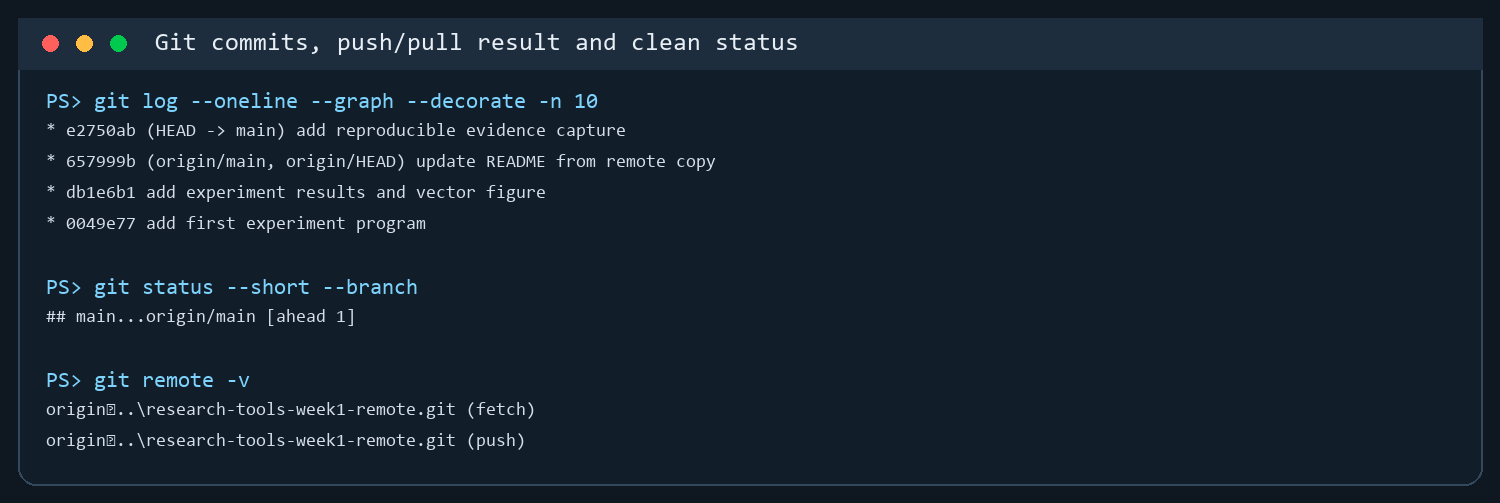
\includegraphics[width=0.93\textwidth]{../evidence/03_git_history.png}
  \caption{Git 提交历史及远程同步结果}
  \label{fig:git}
\end{figure}

GitHub 最终上传命令如下，其中用户名和仓库地址必须由本人填写：

\begin{lstlisting}[language=bash,caption={绑定 GitHub 远程仓库}]
git remote set-url origin https://github.com/<username>/research-tools-week1.git
git push -u origin main
\end{lstlisting}

\section{Codex 辅助编程实验}

\subsection{安装与配置检查}

执行 \texttt{codex --version} 已确认 CLI 安装成功。当前 CLI 的 \texttt{codex login status} 返回 \texttt{Not logged in}，但本实验已在 Codex 桌面应用会话中完成。根据官方文档，CLI 可执行 \texttt{codex login} 通过浏览器使用 ChatGPT 登录，也可通过标准输入使用 API Key；不应把密钥直接写入脚本、配置截图或仓库。安全的基础配置示例如下：

\begin{lstlisting}[language=toml,caption={Codex 基础配置示例}]
model_reasoning_effort = "medium"
approval_policy = "on-request"
sandbox_mode = "workspace-write"
cli_auth_credentials_store = "keyring"
\end{lstlisting}

其中，\texttt{workspace-write} 将写入范围限制在工作区，\texttt{on-request} 在需要越界时请求批准。OpenAI 官方沙盒说明也将这一组合作为较低风险的本地工作方式。\footnote{OpenAI Codex Sandbox: \url{https://learn.chatgpt.com/docs/sandboxing}。访问日期：2026-09-23。}

\subsection{一次明确的 Codex 任务}

本次给 Codex 的任务可概括为：阅读实验要求，创建一个 UTF-8 文本词频统计程序，加入自动测试，运行程序并生成可供 LaTeX 引用的矢量结果图。Codex 生成并修改了 \texttt{code/text\_stats.py}、\texttt{code/test\_text\_stats.py} 和报告文件；随后实际运行程序及测试，并通过 Git 差异与提交历史核对修改。

程序采用正则表达式提取英文单词、数字及汉字，英文统一转为小写，再用 \texttt{Counter} 统计。它只依赖 Python 标准库，CSV 使用 UTF-8 with BOM，便于在常见表格软件中查看。

\begin{lstlisting}[language=Python,caption={词频统计核心逻辑}]
TOKEN_PATTERN = re.compile(r"[A-Za-z0-9_]+|[\u4e00-\u9fff]")

def tokenize(text: str) -> list[str]:
    return [token.lower() for token in TOKEN_PATTERN.findall(text)]

def count_words(text: str) -> Counter[str]:
    return Counter(tokenize(text))
\end{lstlisting}

图~\ref{fig:test} 显示程序读取样例文本后统计出 59 个词元、44 个不同词元，并将前 10 项写入 CSV；三个自动测试全部通过。

\begin{figure}[H]
  \centering
  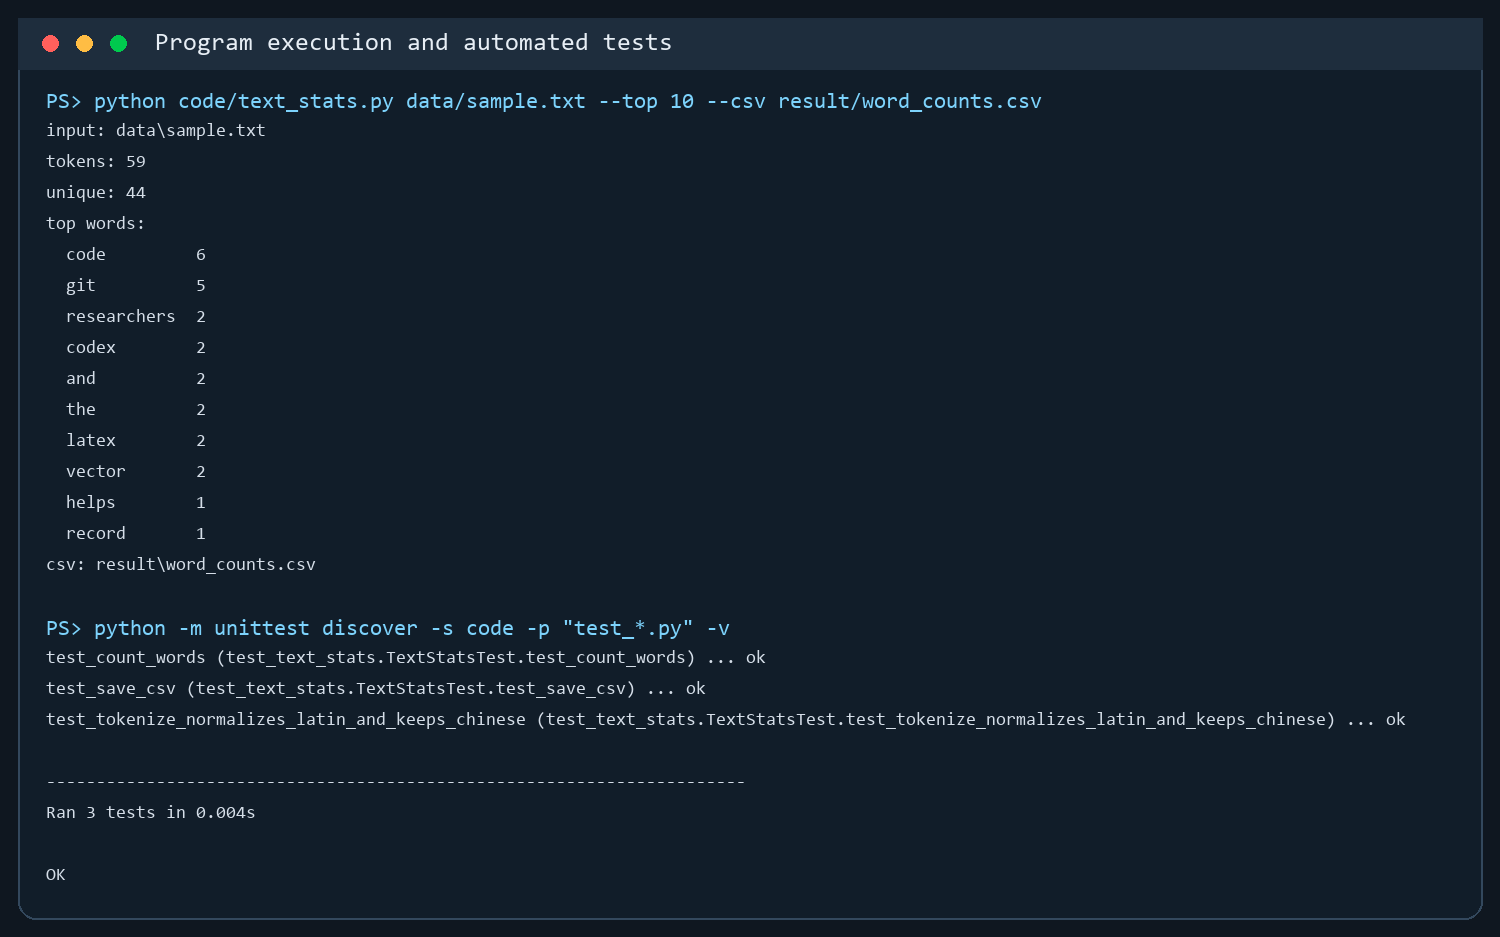
\includegraphics[width=0.93\textwidth]{../evidence/02_program_and_tests.png}
  \caption{程序运行与自动测试结果}
  \label{fig:test}
\end{figure}

\section{CC Switch 安装与供应商切换说明}

本实验从 CC Switch 项目唯一官方 GitHub Releases 下载 Windows 便携版 3.20.4，解压后验证 \texttt{cc-switch.exe} 的产品版本为 3.20.4。下载包 SHA-256 为：

\begin{center}
\small\ttfamily 227288532BFD4F3894D7D9916A8CF340D49957618D8E520229D30BDCC9F5B5D3
\end{center}

项目发布页说明便携版无需写入注册表，官方渠道为 GitHub 项目与 \url{https://ccswitch.io}。\footnote{CC Switch v3.20.4 Release: \url{https://github.com/farion1231/cc-switch/releases/tag/v3.20.4}。访问日期：2026-09-23。}

\begin{figure}[H]
  \centering
  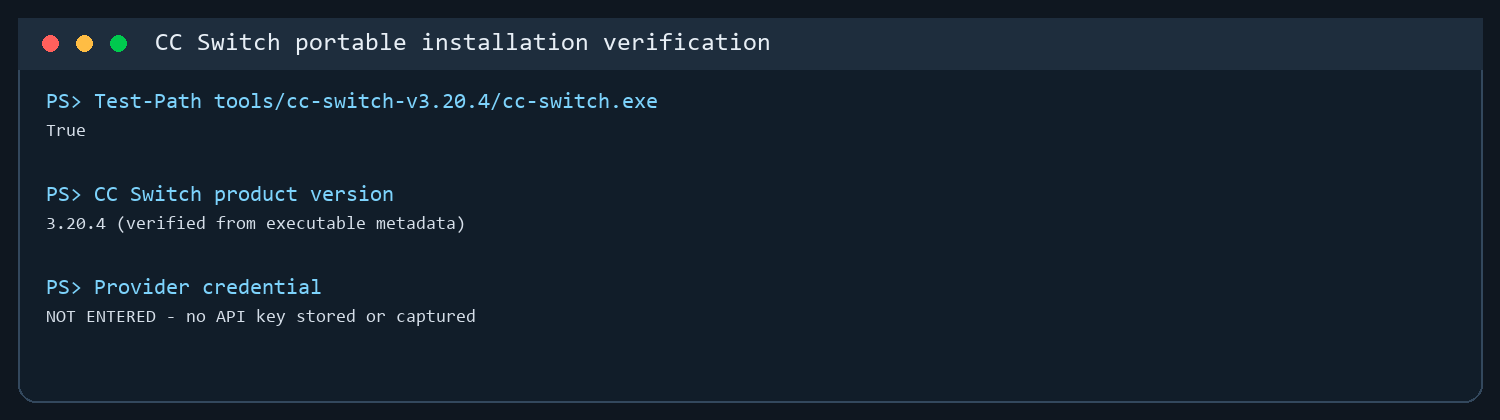
\includegraphics[width=0.90\textwidth]{../evidence/04_cc_switch.png}
  \caption{CC Switch 便携版安装验证（无密钥）}
  \label{fig:ccswitch}
\end{figure}

实际配置供应商时，应在 CC Switch 的 Codex 页面选择“添加供应商”，优先采用内置预设；自定义条目需要供应商名称、Endpoint URL、模型和本人 API Key。保存后启用该卡片，重启 Codex，再用 \texttt{/status} 和一个简单问题验证。由于 API Key 属于个人敏感凭据，本次自动生成的材料没有填写、保存或截图任何密钥，也没有伪造一次成功的第三方请求。提交前由学生本人在受信任环境完成一次供应商启用，并只截取不含密钥的供应商名称与成功状态即可。

\section{结果分析}

\begin{longtable}{p{3.2cm}p{10.5cm}}
  \toprule
  检查项 & 结果 \\
  \midrule
  \endfirsthead
  \toprule
  检查项 & 结果 \\
  \midrule
  \endhead
  程序可运行性 & 词频程序成功输出统计摘要和 CSV，退出状态正常。 \\
  自动测试 & 三个测试覆盖分词归一化、计数和 CSV 写入，全部通过。 \\
  图像规范 & 实验图为 PDF 矢量图，具有图号、图题和正文引用。 \\
  Git 版本管理 & 已完成至少两次功能明确的提交，并验证 push、远程修改和 pull。 \\
  Codex 使用 & 已在当前 Codex 桌面任务中完成代码生成、测试、结果制作和报告整理。 \\
  凭据保护 & 仓库忽略密钥、环境文件和 Codex 私有配置；截图均已脱敏。 \\
  \bottomrule
\end{longtable}

\section{实验总结}

本实验建立了“开始工作先同步、修改后检查差异、测试通过再提交、完成后推送”的基本节奏。Git 的工作区、暂存区、本地仓库和远程仓库具有不同职责，\texttt{status}、\texttt{diff} 与 \texttt{log} 能够提供可审计证据。Codex 能显著提高代码生成和报告整理效率，但输出仍需通过测试和 Git 差异验证。LaTeX 的 \texttt{includegraphics}、\texttt{caption}、\texttt{label} 与 \texttt{ref} 可以形成规范、可维护的图文引用关系。CC Switch 适合管理多个供应商，但增加了本地代理和凭据管理环节，因此必须坚持只使用官方渠道、不公开密钥、切换后重新验证的原则。

\section*{提交前本人确认清单}

\begin{itemize}[leftmargin=2.5em]
  \item 在封面补充姓名、学号和班级；
  \item 在 GitHub 新建 \texttt{research-tools-week1}，替换远程 URL 并推送；
  \item 用本人账号完成 Codex 登录，截图时裁掉邮箱、令牌和密钥；
  \item 在 CC Switch 中启用一个本人有权使用的供应商，重启 Codex 验证；
  \item 将上述两张个人操作截图替换或补入报告，再编译两遍以更新目录和交叉引用。
\end{itemize}

\appendix
\section{复现实验命令}

\begin{lstlisting}[language=bash]
python code/text_stats.py data/sample.txt --top 10 --csv result/word_counts.csv
python -m unittest discover -s code -p "test_*.py" -v
python code/make_figure.py
cd report
xelatex -interaction=nonstopmode -halt-on-error main.tex
xelatex -interaction=nonstopmode -halt-on-error main.tex
\end{lstlisting}

\end{document}
